\documentclass[xcolor=dvipsnames]{beamer}
\usetheme{metropolis}
\usefonttheme{professionalfonts}
\usepackage{algorithm, algpseudocode}
\usepackage{tikz}
\usetikzlibrary{matrix, shapes, fit, calc, backgrounds, chains, positioning, scopes, patterns, patterns.meta, automata, pgfplots.groupplots, plotmarks}
\usepackage{fontawesome}
\usepackage{xcolor}
\usepackage{tabularx}
\usepackage{pgfplots}
\usepgfplotslibrary{groupplots}
\usepackage{pgfplotstable}
\pgfplotsset{compat=1.7}
\usepackage{graphicx}
\usepackage[absolute,overlay]{textpos}
\graphicspath{ {./res/} }
\usepackage{booktabs}
\usepackage{makecell}
\usepackage{blindtext}

%Information to be included in the title page:
\title{Optimizing Write-Heavy Database Operations Using B$^\varepsilon$-Trees}
\author{Christoph Rotte}
\date{September 1, 2022}
\institute{
	Bachelor's Thesis - Final Presentation
	\and
	Chair for Database Systems | Technical University of Munich
}

\begin{document}
	
\frame{\titlepage}
%
\begin{frame}
\frametitle{B/B$^+$-Trees in Databases}

\begin{center}
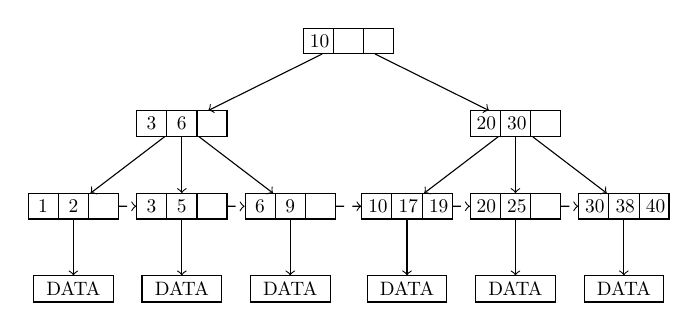
\begin{tikzpicture}[scale=0.7, transform shape]
	\tikzstyle{treenode}=[
	draw,
	rectangle split,
	rectangle split horizontal,
	rectangle split parts=3,
	text width=2ex,
	text centered
	]
	\tikzstyle{datanode}=[
	draw,
	rectangle,
	text centered,
	text width=8ex
	]
	\tikzstyle{level 1}=[sibling distance=40ex]
	\tikzstyle{level 2}=[sibling distance=13ex]
	\node[treenode] {10 \nodepart{two} \nodepart{three}} [->]
	child {node[treenode] {3 \nodepart{two} 6 \nodepart{three}}
		child {node[treenode] (A) {1 \nodepart{two} 2 \nodepart{three}}
			child {node[datanode] {DATA}}
		}
		child {node[treenode] (B) {3 \nodepart{two} 5 \nodepart{three}}
			child {node[datanode] {DATA}}
		}
		child {node[treenode] (C) {6 \nodepart{two} 9 \nodepart{three}}
			child {node[datanode] {DATA}}
		}    
	} 
	child {node[treenode] {20 \nodepart{two} 30 \nodepart{three}}
		child {node[treenode] (D) {10 \nodepart{two} 17 \nodepart{three} 19}
			child {node[datanode] {DATA}}
		}
		child {node[treenode] (E) {20 \nodepart{two} 25 \nodepart{three}}
			child {node[datanode] {DATA}}
		}  
		child {node[treenode] (F) {30 \nodepart{two} 38 \nodepart{three} 40}
			child {node[datanode] {DATA}}
		}     
	};
	\path [->, dashed] (A) edge [right] (B);
	\path [->, dashed] (B) edge [right] (C);
	\path [->, dashed] (C) edge [right] (D);
	\path [->, dashed] (D) edge [right] (E);
	\path [->, dashed] (E) edge [right] (F);
\end{tikzpicture}
\end{center}
\end{frame}
%
% 
\begin{frame}
	\frametitle{B/B$^+$-Trees in Databases}
	
	\begin{center}
		\begin{tikzpicture}[scale=0.7, transform shape]
			\tikzstyle{treenode}=[
			draw,
			rectangle split,
			rectangle split horizontal,
			rectangle split parts=3,
			text width=2ex,
			text centered
			]
			\tikzstyle{datanode}=[
			draw,
			rectangle,
			text centered,
			text width=8ex
			]
			\tikzstyle{level 1}=[sibling distance=40ex]
			\tikzstyle{level 2}=[sibling distance=13ex]
			\node[treenode] (ROOT) {10 \nodepart{two} \nodepart{three}} [->]
			child {node[treenode] (LEFT) {3 \nodepart{two} 6 \nodepart{three}}
				child {node[treenode] (A) {1 \nodepart{two} 2 \nodepart{three}}
					child {node[datanode] {DATA}}
				}
				child {node[treenode] (B) {3 \nodepart{two} 5 \nodepart{three}}
					child {node[datanode] {DATA}}
				}
				child {node[treenode] (C) {6 \nodepart{two} 9 \nodepart{three}}
					child {node[datanode] {DATA}}
				}    
			} 
			child {node[treenode] (RIGHT) {20 \nodepart{two} 30 \nodepart{three}}
				child {node[treenode] (D) {10 \nodepart{two} 17 \nodepart{three} 19}
					child {node[datanode] {DATA}}
				}
				child {node[treenode] (E) {20 \nodepart{two} 25 \nodepart{three}}
					child {node[datanode] {DATA}}
				}  
				child {node[treenode] (F) {30 \nodepart{two} 38 \nodepart{three} 40}
					child {node[datanode] {DATA}}
				}     
			};
			\path [->, dashed] (A) edge [right] (B);
			\path [->, dashed] (B) edge [right] (C);
			\path [->, dashed] (C) edge [right] (D);
			\path [->, dashed] (D) edge [right] (E);
			\path [->, dashed] (E) edge [right] (F);
			%
			\node[draw=red, fit=(ROOT), label=left:{\color{red} \faLock { (r/w) Page 3}}, text=red] {};
			\node[draw=red, fit=(RIGHT), label=left:{\color{red} \faLock { (r/w) Page 4}}, text=red] {};
		\end{tikzpicture}
	\end{center}
\end{frame}
% 
\begin{frame}
	\frametitle{Log-Structured Merge-Trees (LSM-Trees)}
	
	\begin{center}
		\vspace*{7mm}
		\scalebox{0.7}{
		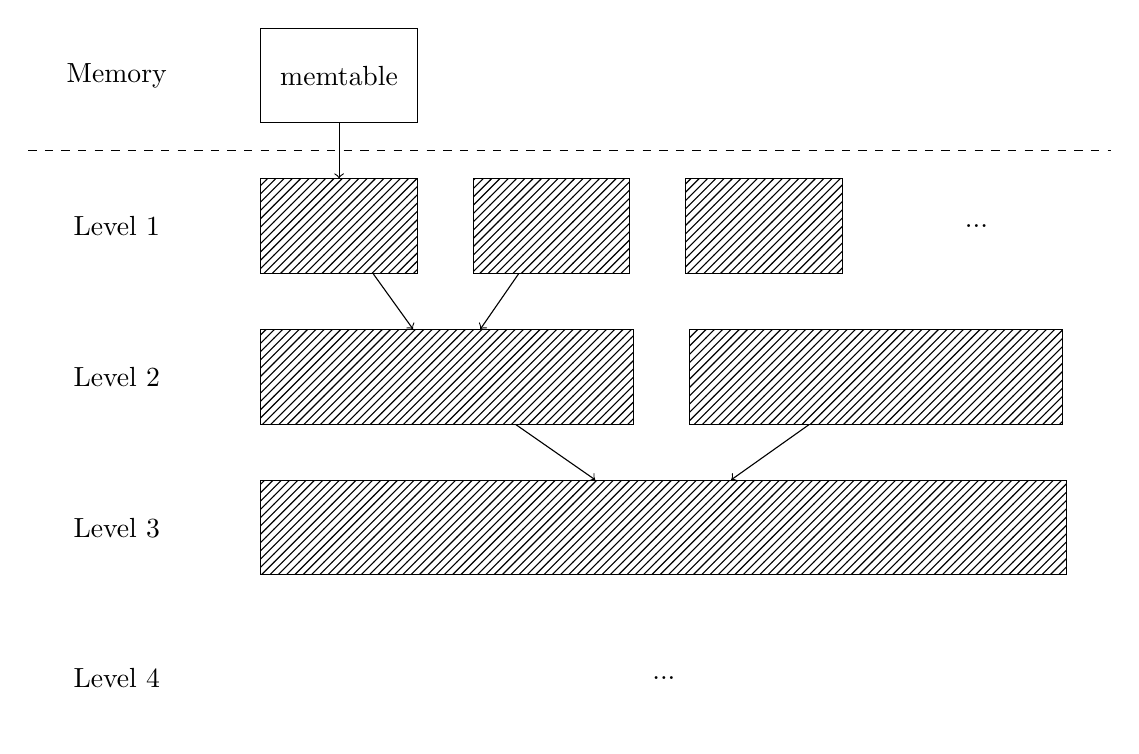
\begin{tikzpicture}[
			node distance=7mm,
			default_node/.style={
				rectangle,
				draw=black, 
				%very thick,
				text centered,
				minimum height=12mm,
				pattern=north east lines,
				pattern color=black
			},
			empty_node/.style={
				rectangle,
				draw=none, 
				%very thick,
				text centered,
				minimum height=12mm
			},
			desc/.style={
				minimum height=12mm,
				text width=2cm,
				text centered
			},
			line/.style={
				->,
				%very thick
			}
			]
			
			% Descriptions
			
			\node [desc] (D0) {Memory};
			\node [desc, below=of D0] (D1) {Level 1};
			\node [desc, below=of D1] (D2) {Level 2};
			\node [desc, below=of D2] (D3) {Level 3};
			\node [desc, below=of D3] (D4) {Level 4};
			
			% Levels
			
			\node [default_node, pattern=none, text width=1.75cm, right=of D0] (memtable) {memtable};
			
			\node [default_node, text width=1.75cm, right=of D1] (L1_1) {};
			\node [default_node, text width=1.75cm, right=of L1_1] (L1_2) {};
			\node [default_node, text width=1.75cm, right=of L1_2] (L1_3) {};
			\node [empty_node, text width=1.75cm, right=of L1_3] (L1_4) {...};
			
			\node [default_node, text width=4.5cm, right=of D2] (L2_1) {};
			\node [default_node, text width=4.5cm, right=of L2_1] (L2_2) {};
			
			\node [default_node, text width=10cm, right=of D3] (L3) {};
			
			\node [default_node, text width=10cm, draw=none, pattern=none, right=of D4] (L4) {...};
			
			% Connections
			
			\draw[line] (memtable.south -| L1_1.north) -- (L1_1.north);
			
			\path [line] (L1_1) edge [below] (L2_1);
			\path [line] (L1_2) edge [below] (L2_1);
			
			\path [line] (L2_1) edge [below] (L3);
			\path [line] (L2_2) edge [below] (L3);
			
			% Separator
			
			\draw[dashed] let \p1=(D0),\p2=(D1),\p3=(D1.north west),\p4=(D1.north east) in 
			(\x3,{(\y1+\y2)/2}) -- (\x4+11.5cm,{(\y1+\y2)/2});
			
		\end{tikzpicture}
		}
	\end{center}
\end{frame}
% 

\newcommand\Textbox[2]{%
	\parbox[c][#1][c]{2.3cm}{\centering#2}}

\begin{frame}
	\frametitle{B$^\varepsilon$-Trees | Structure}
	
	\begin{center}
		\vspace*{3mm}
		\scalebox{0.68}{
			\begin{tikzpicture}[
				inner_node/.style={
					rectangle split,
					rectangle split horizontal=false,
					draw=black,
					rectangle split ignore empty parts,
					rectangle split part align={left},
					text centered
				},
				inner/.style={
					rectangle split horizontal,
					draw=black,
					rectangle split ignore empty parts,
					rectangle split part align={center,base},
					rectangle split parts=20,
					text centered
				},
				dotted_node/.style={
					rectangle,
					draw=none, 
					text centered,
					align=center,
					text width=2cm, 
					text height=0.5cm, 
					text depth=0.5cm
				},
				edge from parent/.style={->, draw}
				]
				
				\node[inner_node] (ROOT) {
					\begin{tikzpicture}
						\node[inner, label=right:$B-B^\varepsilon$] (BUFFER) {
							\Textbox{1cm}{upsert buffer}
						};
						
					\end{tikzpicture}
					\nodepart{two} \begin{tikzpicture}
						\node[inner, label={[label distance=1.5mm]right:$B^\varepsilon$}] (ROOT_pivots)
						{$P_1$\nodepart{two}$P_2$\nodepart{three}$P_3$\nodepart{four}$P_4$\nodepart{five}...};
					\end{tikzpicture}
				};
				
				\node[inner_node, below=of ROOT] (L_1_CENTER) {
					\begin{tikzpicture}
						\node[inner, label=right:$B-B^\varepsilon$] (BUFFER) {
							\Textbox{1cm}{upsert buffer}
						};
						
					\end{tikzpicture}
					\nodepart{two} \begin{tikzpicture}
						\node[inner, label={[label distance=1.5mm]right:$B^\varepsilon$}] (ROOT_pivots)
						{$P_1$\nodepart{two}$P_2$\nodepart{three}$P_3$\nodepart{four}$P_4$\nodepart{five}...};
					\end{tikzpicture}
				};
				
				\node[dotted_node, left=of L_1_CENTER] (L_1_2){
					...
				};
				
				\node[dotted_node, right=of L_1_CENTER] (L_1_3){
					...
				};
				
				\node[dotted_node, below=of L_1_CENTER] (L_2_CENTER){
					...
				};
				
				\node[dotted_node, left=of L_2_CENTER] (L_2_1){
					...
				};
				
				\node[dotted_node, right=of L_2_CENTER] (L_2_2){
					...
				};
				
				\node[inner_node, below=of L_2_CENTER] (LEAF_CENTER) {
					\begin{tikzpicture}
						\node[inner, label={[label distance=1.5mm]right:$B$}] (ROOT_pivots)
						{$(K_1,V_{K_1})$\nodepart{two}$(K_2,V_{K_2})$\nodepart{three}$(K_3,V_{K_3})$\nodepart{four}$(K_4,V_{K_4})$\nodepart{five}$(K_5,V_{K_5})$\nodepart{six}$(K_6,V_{K_6})$\nodepart{seven}...};
					\end{tikzpicture}
				};
				
				\path [->] (ROOT) edge [below] (L_1_2);
				\path [->] (ROOT) edge [below] (L_1_CENTER);
				\path [->] (ROOT) edge [below] (L_1_3);
				
				\path [->] (L_1_CENTER) edge [below] (L_2_1);
				\path [->] (L_1_CENTER) edge [below] (L_2_CENTER);
				\path [->] (L_1_CENTER) edge [below] (L_2_2);
				
				\path [->] (L_2_CENTER) edge [below] (LEAF_CENTER);
				
			\end{tikzpicture}
		}
	\end{center}
\end{frame}

\begin{frame}
	\frametitle{B$^\varepsilon$-Trees | Lookups}
	
	\begin{center}
		\vspace*{5mm}
		\scalebox{0.75}{
			\begin{tikzpicture}[
				inner_node/.style={
					rectangle split,
					rectangle split horizontal=false,
					draw=black,
					rectangle split ignore empty parts,
					rectangle split part align={center,base},
					text centered
				},
				inner/.style={
					rectangle split horizontal,
					draw=black,
					rectangle split ignore empty parts,
					rectangle split part align={center,base},
					rectangle split parts=20,
					text centered
				},
				dotted_node/.style={
					rectangle,
					draw=none, 
					text centered,
					align=center,
					text width=2cm, 
					text height=0.5cm, 
					text depth=0.5cm
				},
				edge from parent/.style={->, draw}
				]
				
				\node[inner_node] (ROOT) {
					\begin{tikzpicture}
						\node[inner, rectangle split part fill={white,red!30,white!30,red!30,red!30,white}] (ROOT_pivots)
						{...\nodepart{two}$U_3^K$\nodepart{three}...\nodepart{four}$U_4^K$\nodepart{five}$U_5^K$\nodepart{six}...};
					\end{tikzpicture}
					\nodepart{two} \begin{tikzpicture}
						\node[inner] (ROOT_pivots)
						{$P_1$\nodepart{two}$P_2$\nodepart{three}$P_3$\nodepart{four}$P_4$\nodepart{five}...};
					\end{tikzpicture}
				};
				
				\node[inner_node, below=of ROOT] (L_1_CENTER) {
					\begin{tikzpicture}
						\node[inner, rectangle split part fill={white,red!30,white,red!30,white}] (ROOT_pivots)
						{...\nodepart{two}$U_1^K$\nodepart{three}...\nodepart{four}$U_2^K$\nodepart{five}...};
					\end{tikzpicture}
					\nodepart{two} \begin{tikzpicture}
						\node[inner] (ROOT_pivots)
						{$P_1$\nodepart{two}$P_2$\nodepart{three}$P_3$\nodepart{four}$P_4$\nodepart{five}...};
					\end{tikzpicture}
				};
				
				\node[dotted_node, left=of L_1_CENTER] (L_1_2){
					...
				};
				
				\node[dotted_node, right=of L_1_CENTER] (L_1_3){
					...
				};
				
				\node[dotted_node, below=of L_1_CENTER] (L_2_CENTER){
					...
				};
				
				\node[dotted_node, left=of L_2_CENTER] (L_2_1){
					...
				};
				
				\node[dotted_node, right=of L_2_CENTER] (L_2_2){
					...
				};
				
				\node[inner_node, below=of L_2_CENTER] (LEAF_CENTER) {
					\begin{tikzpicture}
						\node[inner, rectangle split part fill={white,red!30,white}] (ROOT_pivots)
						{...\nodepart{two}$(K,V_K)$\nodepart{three}...};
					\end{tikzpicture}
				};
				
				\path [->] (ROOT) edge [below] (L_1_2);
				\path [->, draw=red] (ROOT) edge [below] (L_1_CENTER);
				\path [->] (ROOT) edge [below] (L_1_3);
				
				\path [->] (L_1_CENTER) edge [below] (L_2_1);
				\path [->, draw=red] (L_1_CENTER) edge [below] (L_2_CENTER);
				\path [->] (L_1_CENTER) edge [below] (L_2_2);
				
				\path [->, draw=red] (L_2_CENTER) edge [below] (LEAF_CENTER);
				
				\draw[->, color=red] (-5,1) -- (-5,-7.5) node[sloped,midway,below] {};
				\draw[->, color=darkgray] (5,-7.5) -- (5,1) node[sloped,midway,above,rotate=180] {};
				
			\end{tikzpicture}
		}
	\end{center}
\end{frame}

\begin{frame}
	\frametitle{Asymptotic Comparison | I/O Operations}
	
	\begin{table}[h]
		\centering
		\vspace*{5mm}
		\scalebox{1.1}{
		\begin{tabular}{@{}llll@{}}
			\toprule
			& B/B$^+$-Tree         & B$^\varepsilon$-Tree                                & LSM-Tree                                            \\ \midrule
			\addlinespace[2mm]
			Upserts       & \makecell{\textcolor{red}{$-$}}               & \makecell{\textcolor{teal}{$+$}}  & \makecell{\textcolor{teal}{$+$}}  \\
			\addlinespace[2mm]
			Lookups & \makecell{\textcolor{teal}{$+$}}               & \makecell{\textcolor{orange}{$+$}}                   & \makecell{\textcolor{red}{$-$}}                 \\
			\addlinespace[2mm]
			\bottomrule
		\end{tabular}
		}
	\end{table}
\end{frame}

\begin{frame}
	\frametitle{Implementation | Preemptive Splitting}
	\begin{center}
		\scalebox{0.65}{
			\hspace*{-8mm}
			\begin{tikzpicture}[
				inner_node/.style={
					rectangle split,
					rectangle split horizontal=false,
					draw=black,
					rectangle split ignore empty parts,
					rectangle split part align={center,base},
					text centered
				},
				inner/.style={
					rectangle split horizontal,
					draw=black,
					rectangle split ignore empty parts,
					rectangle split part align={center,base},
					rectangle split parts=20,
					text centered
				},
				dotted_node/.style={
					rectangle,
					draw=none, 
					text centered,
					align=center,
					text width=0.25cm, 
					text height=0.5cm, 
					text depth=0.5cm
				},
				edge from parent/.style={->, draw}
				]
				
				\node[dotted_node] (ROOT) {
					...
				};
				
				\node[inner_node, below=of ROOT] (CENTER) {
					\begin{tikzpicture}
						\node[inner, rectangle split part fill={white,white,white,blue!20}] (ROOT_pivots)
						{$U^{K_1}_1$\nodepart{two}$U^{K_2}_1$\nodepart{three}$U^{K_3}_1$\nodepart{four}$U^{K_4}_1$\nodepart{five}$U^{K_4}_2$};
					\end{tikzpicture}
					\nodepart{two} \begin{tikzpicture}
						\node[inner] (ROOT_pivots)
						{1\nodepart{two}2\nodepart{three}3};
					\end{tikzpicture}
				};
				
				\node[dotted_node, below=of CENTER, xshift=-0.8cm] (child2) {
					...
				};
				\node[dotted_node, left=of child2] (child1) {
					...
				};
				\node[dotted_node, right=of child2] (child3) {
					...
				};
				\node[dotted_node, right=of child3] (child3_1) {
					...
				};
				
				\path [->, draw=blue] (ROOT) edge [below] (CENTER);
				
				\path [->] (CENTER) edge [below] (child1);
				%\path [->, dotted, thick] (child2) edge [below, bend right] node[midway, right, draw=black, solid, xshift=1mm, semithick] {2} (CENTER);
				\path [->] (CENTER) edge [below] (child2);
				\path [->] (CENTER) edge [below] (child3);
				\path [->, draw=blue] (CENTER) edge [below] (child3_1);
				
				% ------------------------------------------------------------
				
				\node[inner_node, right=of CENTER, xshift=0.5cm] (CENTER2) {
					\begin{tikzpicture}
						\node[inner] (ROOT_pivots)
						{$U^{K_1}_1$\nodepart{two}$U^{K_2}_1$\nodepart{three}\phantom{$U^{K_3}_1$}\nodepart{four}\phantom{$U^{K_4}_1$}\nodepart{five}\phantom{$U^{K_4}_2$}};
					\end{tikzpicture}
					\nodepart{two} \begin{tikzpicture}
						\node[inner] (ROOT_pivots)
						{1\nodepart{two}\phantom{3}\nodepart{three}\phantom{1}};
					\end{tikzpicture}
				};
				
				\node[inner_node, right=of CENTER2, xshift=-0.5cm] (CENTER3) {
					\begin{tikzpicture}
						\node[inner] (ROOT_pivots)
						{$U^{K_3}_1$\nodepart{two}\phantom{$U^{K_4}_1$}\nodepart{three}\phantom{$U^{K_4}_2$}\nodepart{four}\phantom{$U^{K_4}_1$}\nodepart{five}\phantom{$U^{K_4}_2$}};
					\end{tikzpicture}
					\nodepart{two} \begin{tikzpicture}
						\node[inner] (ROOT_pivots)
						{3\nodepart{two}\phantom{3}\nodepart{three}\phantom{1}};
					\end{tikzpicture}
				};
				
				\node[dotted_node, above=of CENTER2, text width=2cm, xshift=2.85cm] (ROOT2) {
					... 2 ...
				};
				
				\node[dotted_node, below=of CENTER2, xshift=-0.75cm] (child4) {
					...
				};
				\node[dotted_node, right=of child4] (child5) {
					...
				};
				
				\node[dotted_node, below=of CENTER3, xshift=-0.75cm] (child6) {
					...
				};
				\node[dotted_node, right=of child6] (child7) {
					...
				};
				
				\path [->] (ROOT2) edge [below] (CENTER2);
				\path [->] (ROOT2) edge [below] (CENTER3);
				
				\path [->] (CENTER2) edge [below] (child4);
				\path [->] (CENTER2) edge [below] (child5);
				
				\path [->] (CENTER3) edge [below] (child6);
				\path [->] (CENTER3) edge [below] (child7);
				
				% ------------------------------------------------------------
				
				\draw[->, color=darkgray, very thick] (2.9,-2.6) -- (3.5,-2.6);
				
			\end{tikzpicture}
		}
	\end{center}
	
\end{frame}

\begin{frame}
	\frametitle{Implementation | Separate Root Node}
\begin{center}
	
	\scalebox{0.7}{
		\begin{tikzpicture}[
			inner_node/.style={
				rectangle split,
				rectangle split horizontal=false,
				draw=black,
				rectangle split ignore empty parts,
				rectangle split part align={center,base},
				text centered
			},
			inner/.style={
				rectangle split horizontal,
				draw=black,
				rectangle split ignore empty parts,
				rectangle split part align={center,base},
				rectangle split parts=20,
				text centered
			},
			dotted_node/.style={
				rectangle,
				draw=none, 
				text centered,
				align=center,
				text width=1cm, 
				text height=1cm, 
				text depth=1cm
			},
			edge from parent/.style={->, draw}
			]
			
			\node[inner_node] (ROOT) {
				\begin{tikzpicture}
					\node[inner] (ROOT_pivots)
					{$K_1$\nodepart{two}$K_2$\nodepart{three}$K_3$\nodepart{four}$K_4$\nodepart{five}$K_5$\nodepart{six}$K_6$\nodepart{seven}$K_7$\nodepart{eight}$K_8$\nodepart{nine}$K_9$\nodepart{ten}...};
				\end{tikzpicture}
			};
			
			\node[inner_node, below=of ROOT, yshift=-1cm] (child1) {
				\begin{tikzpicture}
					\node[inner] (ROOT_pivots){upsert buffer};
				\end{tikzpicture}
				\nodepart{two} \begin{tikzpicture}
					\node[inner] (ROOT_pivots){pivots};
				\end{tikzpicture}
			};
			
			\node[dotted_node, left=of child1] (child2) {
				\textcolor{gray}{...}
			};
			
			\node[inner_node, left=of child2] (child3) {
				\begin{tikzpicture}
					\node[inner] (ROOT_pivots){upsert buffer};
				\end{tikzpicture}
				\nodepart{two} \begin{tikzpicture}
					\node[inner] (ROOT_pivots){pivots};
				\end{tikzpicture}
			};
			
			\node[dotted_node, right=of child1] (child4) {
				\textcolor{gray}{...}
			};
			
			\node[inner_node, right=of child4, draw=gray] (child5) {
				\begin{tikzpicture}
					\node[inner, draw=gray] (ROOT_pivots){\textcolor{gray}{upsert buffer}};
				\end{tikzpicture}
				\nodepart{two} \begin{tikzpicture}
					\node[inner, draw=gray] (ROOT_pivots){\textcolor{gray}{pivots}};
				\end{tikzpicture}
			};
			
			\path [->] (ROOT) edge [below] node[midway, draw=none, fill=normal text.bg] {$T_2$} (child1);
			\path [->, draw=gray] (ROOT) edge [below] (child2);
			\path [->] (ROOT) edge [below] node[midway, draw=none, fill=normal text.bg, xshift=-5mm] {$T_1$} (child3);
			\path [->, draw=gray] (ROOT) edge [below] (child4);
			\path [->, draw=gray] (ROOT) edge [below] (child5);
			
			\node[draw=red, fit=(ROOT), label=above:{\color{red} \faLock { (T1, T2: shared) }}, text=red] {};
			\node[draw=blue, fit=(child3), label=below:{\color{blue} \faLock { (T1: exclusive) }}, text=blue] {};
			\node[draw=blue, fit=(child1), label=below:{\color{blue} \faLock { (T2: exclusive) }}, text=blue] {};
			
			%\path [->, dotted, thick] (child2) edge [below, bend right] node[midway, right, draw=black, solid, xshift=1mm, semithick] {2} (CENTER);
			
		\end{tikzpicture}
	}
	
\end{center}
\end{frame}

\begin{frame}
\frametitle{Implementation | Design Layers}

\begin{center}
\scalebox{0.67}{
	\hspace*{-1.3cm}
	\begin{tikzpicture}[
		node distance=7mm,
		default_node/.style={
			rectangle,
			draw=black, 
			text centered,
			minimum width=12mm,
			minimum height=12mm,
			text width=3cm
		},
		desc/.style={
			minimum height=2cm,
			text width=2.5cm,
			text centered,
			align=center,
			draw=none
		},
		line/.style={
			<->,
		}
		]
		
		% Descriptions
		
		%\node [desc, minimum height=5mm] (D0) {\textbf{Main Interfaces}};
		\node [desc, below=of D0] (D1) {
			\texttt{insert()}
			\texttt{update()}
			\texttt{erase()}
			\texttt{find()}
		};
		\node [desc, below=of D1] (D2) {
			\texttt{createPage()}
			\texttt{deletePage()}
			\texttt{pinPage()}
			\texttt{unpinPage()}
		};
		\node [desc, below=of D2] (D3) {
			\texttt{createBlock()}
			\texttt{deleteBlock()}
			\texttt{readBlock()}
			\texttt{writeBlock()}
		};
		\node [desc, below=of D3] (D4) {
			\texttt{glibc:}
			\texttt{\textcolor{gray}{pread()}}
			\texttt{\textcolor{gray}{pwrite()}}
			\texttt{\textcolor{gray}{ftruncate()}}
		};
		
		% Levels
		
		\node [default_node, left=of D1] (tree) {B$^\varepsilon$-Tree \& B$^+$-Tree};
		\node [default_node, left=of D2] (buffer) {2Q Page Buffer};
		\node [default_node, left=of buffer] (buffer2) {"Optimal" Page Buffer};
		\node [default_node, left=of D3] (segments) {Segment Manager};
		\node [default_node, left=of D4] (disk) {Disk Storage};
		
		\path [line] (tree) edge [below] (buffer);
		\path [line] (buffer) edge [below] (segments);
		\path [line] (segments) edge [below] (disk);
		
	\end{tikzpicture}
}
\end{center}

\end{frame}

\begin{frame}
\frametitle{Evaluation | Benchmark Setup}

\vspace*{4mm}
\begin{center}
	\begin{itemize}
		\item \textbf{Benchmark Tool}: Unum Cloud Benchmark (UCSB)\newline
		\hspace*{30mm}$\rightarrow$ rewrite of YCSB in C++
		\item Intel i9-7900X (20 threads) | Samsung SSD 970 EVO
		\item \textbf{Sizes}: 16KiB pages | 8B keys | 100B values
		\item \textbf{Distribution}: Zipfian (constant: $0.99$)
	\end{itemize}
\end{center}	
\end{frame}


\newcommand{\verticalplotscale}{0.89}
\begin{frame}
\frametitle{"Optimal" Buffer | 200M Operations w/ 200M Preloaded Values}
\begin{center}
\vspace*{-5mm}
\hspace*{-5mm}
\scalebox{0.7}{
	\begin{tikzpicture}[
		desc/.style={
			minimum height=2cm,
			text width=2.5cm,
			text centered,
			align=center,
			draw=none
		}
		]
		
		\node [desc, yshift=7cm, xshift=1.6cm, darkgray] (NODE1) {
			Buffered Binary Tree ($\varepsilon=0$)
		};
		\node [desc, right= 8cm of NODE1, darkgray] (NODE2) {
			B$^+$-Tree ($\varepsilon=1$)
		};
		\draw[solid, ->, darkgray] (NODE1) to (NODE2);
	
		\begin{groupplot}[
			group style={group size=2 by 1}
			]
			
			\nextgroupplot[
			title=200M Inserts,
			width=\axisdefaultwidth,
			height= \verticalplotscale*\axisdefaultheight,
			xlabel=$\varepsilon$,
			ylabel={Throughput [ops/s]},
			xmin=30, xmax=100,
			ymin=0, ymax=10000000,
			xtick={5, 15, 25, 35, 45, 55, 65, 75, 85, 95},
			xticklabel={\pgfmathparse{\tick/100}\pgfmathprintnumber[precision=2]\pgfmathresult},
			xticklabel style={/pgf/number format/fixed},
			legend to name=main_legend,
			legend style={legend columns=4, /tikz/every even column/.append style={column sep=0.25cm}}
			]
			\coordinate (c1) at (rel axis cs:0,1);
			\addplot +[color=blue, raw gnuplot, mark=square] gnuplot {
				plot 'data/benchmark/1/zipfian/inserts/16.dat' with points;
			};
			\addplot +[color=purple, raw gnuplot, mark=x] gnuplot {
				plot 'data/benchmark/1/uniform/inserts/16.dat' with points;
			};
			\addplot +[color=teal, raw gnuplot, mark=square] gnuplot {
				plot 'data/benchmark/1/zipfian/inserts/1.dat' with points;
			};
			\addplot +[color=orange, raw gnuplot, mark=x] gnuplot {
				plot 'data/benchmark/1/uniform/inserts/1.dat' with points;
			};
			\draw [dashed, color=gray] (80, 0) -- (80, 100) node [left, midway] {$\varepsilon=0.8$};
			\addlegendentry{t=16 (zipfian)};
			\addlegendentry{t=16 (uniform)};
			\addlegendentry{t=1 (zipfian)};
			\addlegendentry{t=1 (uniform)};
			
			\nextgroupplot[
			title=200M Reads,
			width=\axisdefaultwidth,
			height= \verticalplotscale*\axisdefaultheight,
			xlabel=$\varepsilon$,
			xmin=30, xmax=100,
			ymin=0, ymax=10000000,
			xtick={5, 15, 25, 35, 45, 55, 65, 75, 85, 95},
			xticklabel={\pgfmathparse{\tick/100}\pgfmathprintnumber[precision=2]\pgfmathresult},
			xticklabel style={/pgf/number format/fixed}
			]
			\coordinate (c2) at (rel axis cs:1,1);
			\addplot +[color=blue, raw gnuplot, mark=square] gnuplot {
				plot 'data/benchmark/1/zipfian/reads/16.dat' with points;
			};
			\addplot +[color=teal, raw gnuplot, mark=square] gnuplot {
				plot 'data/benchmark/1/zipfian/reads/1.dat' with points;
			};
			\addplot +[color=purple, raw gnuplot, mark=x] gnuplot {
				plot 'data/benchmark/1/uniform/reads/16.dat' with points;
			};
			\addplot +[color=orange, raw gnuplot, mark=x] gnuplot {
				plot 'data/benchmark/1/uniform/reads/1.dat' with points;
			};
			\draw [dashed, color=gray] (80, 0) -- (80, 100) node [left, midway] {$\varepsilon=0.8$};
			
		\end{groupplot}
		
		\coordinate (c3) at ($(c1)!.5!(c2)$);
		\node[below, xshift=-7mm] at (c3 |- current bounding box.south) (DESC){
			\pgfplotslegendfromname{main_legend}
		};
		
		\node[desc, text width=10cm, below= of DESC, yshift=1.1cm, darkgray]{
			$\varepsilon$ = $0.8$ $\rightarrow$ buffer slots = $109$, pivots = $147$
		};
		
	\end{tikzpicture}
}
\end{center}
\end{frame}

\begin{frame}
\frametitle{"Optimal" Buffer | 200M Operations w/ 200M Preloaded Values}
\begin{center}
\vspace*{5mm}
\hspace*{-5mm}
\scalebox{0.7}{
	\begin{tikzpicture}
		\begin{groupplot}[
			group style={group size=2 by 1}
			]
			
			\nextgroupplot[
			title={200M Inserts},
			width=\axisdefaultwidth,
			height= \verticalplotscale*\axisdefaultheight,
			xlabel={Threads},
			ylabel={Throughput [ops/s]},
			xmin=0, xmax=21,
			ymin=0, ymax=10000000,
			xtick={2, 4, 6, 8, 10, 12, 14, 16, 18, 20},
			legend to name=main_legend,
			legend entries={
				B$^\varepsilon$-Tree,
				B$^+$-Tree,
				B$^\varepsilon$-Tree (w/o separate root)
			},
			legend style={legend columns=3, /tikz/every even column/.append style={column sep=0.25cm}}
			]
			\addlegendimage{blue, mark=x}
			\addlegendimage{red, mark=x}
			\addlegendimage{cyan, mark=square}
			\addplot +[color=blue, raw gnuplot, no marks] gnuplot {
				plot 'data/benchmark/2/epsilon_80/inserts_preloaded/b_epsilon.dat' smooth sbezier;
			};
			\addplot +[color=blue, raw gnuplot, only marks, mark=x] gnuplot {
				plot 'data/benchmark/2/epsilon_80/inserts_preloaded/b_epsilon.dat' with points;
			};
			\addplot +[color=cyan, raw gnuplot, no marks] gnuplot {
				plot 'data/benchmark/2/epsilon_80/inserts_preloaded/b_epsilon_root.dat' smooth sbezier;
			};
			\addplot +[color=cyan, raw gnuplot, only marks, mark=square] gnuplot {
				plot 'data/benchmark/2/epsilon_80/inserts_preloaded/b_epsilon_root.dat' with points;
			};
			\addplot +[color=red, raw gnuplot, no marks] gnuplot {
				plot 'data/benchmark/2/epsilon_80/inserts_preloaded/b_plus.dat' smooth sbezier;
			};
			\addplot +[color=red, raw gnuplot, only marks, mark=x] gnuplot {
				plot 'data/benchmark/2/epsilon_80/inserts_preloaded/b_plus.dat' with points;
			};
			
			\nextgroupplot[
			title={200M Reads},
			width=\axisdefaultwidth,
			height= \verticalplotscale*\axisdefaultheight,
			xlabel={Threads},
			xmin=0, xmax=21,
			ymin=0, ymax=10000000,
			xtick={2, 4, 6, 8, 10, 12, 14, 16, 18, 20}
			]
			\addplot +[color=blue, raw gnuplot, no marks] gnuplot {
				plot 'data/benchmark/2/epsilon_80/reads/b_epsilon.dat' smooth sbezier;
			};
			\addplot +[color=blue, raw gnuplot, only marks, mark=x] gnuplot {
				plot 'data/benchmark/2/epsilon_80/reads/b_epsilon.dat' with points;
			};
			\addplot +[color=cyan, raw gnuplot, no marks] gnuplot {
				plot 'data/benchmark/2/epsilon_80/reads/b_epsilon_root.dat' smooth sbezier;
			};
			\addplot +[color=cyan, raw gnuplot, only marks, mark=square] gnuplot {
				plot 'data/benchmark/2/epsilon_80/reads/b_epsilon_root.dat' with points;
			};
			\addplot +[color=red, raw gnuplot, no marks] gnuplot {
				plot 'data/benchmark/2/epsilon_80/reads/b_plus.dat' smooth sbezier;
			};
			\addplot +[color=red, raw gnuplot, only marks, mark=x] gnuplot {
				plot 'data/benchmark/2/epsilon_80/reads/b_plus.dat' with points;
			};
			
		\end{groupplot}
		
		\coordinate (c3) at ($(c1)!.5!(c2)$);
		\node[below, xshift=-7mm] at (c3 |- current bounding box.south){
			\pgfplotslegendfromname{main_legend}
		};
		
	\end{tikzpicture}
}
\end{center}
\end{frame}


\begin{frame}
	\frametitle{"Optimal" Buffer | 200M Operations w/ 200M Preloaded Values}
	\begin{center}
		\vspace*{5mm}
		\hspace*{-5mm}
		\scalebox{0.7}{
			\begin{tikzpicture}
				\begin{groupplot}[
					group style={group size=2 by 1}
					]
					
					\nextgroupplot[
					title={190M Reads, 10M Inserts},
					width=\axisdefaultwidth,
					height= \verticalplotscale*\axisdefaultheight,
					xlabel={Threads},
					ylabel={Throughput [ops/s]},
					xmin=0, xmax=21,
					ymin=0, ymax=10000000,
					xtick={2, 4, 6, 8, 10, 12, 14, 16, 18, 20},
					legend to name=main_legend,
					legend entries={
						B$^\varepsilon$-Tree,
						B$^+$-Tree,
						B$^\varepsilon$-Tree (w/o separate root)
					},
					legend style={legend columns=3, /tikz/every even column/.append style={column sep=0.25cm}}
					]
					\addlegendimage{blue, mark=x}
					\addlegendimage{red, mark=x}
					\addlegendimage{cyan, mark=square}
					\addplot +[color=blue, raw gnuplot, no marks] gnuplot {
						plot 'data/benchmark/2/epsilon_80/95_5/b_epsilon.dat' smooth sbezier;
					};
					\addplot +[color=blue, raw gnuplot, only marks, mark=x] gnuplot {
						plot 'data/benchmark/2/epsilon_80/95_5/b_epsilon.dat' with points;
					};
					\addplot +[color=cyan, raw gnuplot, no marks] gnuplot {
						plot 'data/benchmark/2/epsilon_80/95_5/b_epsilon_root.dat' smooth sbezier;
					};
					\addplot +[color=cyan, raw gnuplot, only marks, mark=square] gnuplot {
						plot 'data/benchmark/2/epsilon_80/95_5/b_epsilon_root.dat' with points;
					};
					\addplot +[color=red, raw gnuplot, no marks] gnuplot {
						plot 'data/benchmark/2/epsilon_80/95_5/b_plus.dat' smooth sbezier;
					};
					\addplot +[color=red, raw gnuplot, only marks, mark=x] gnuplot {
						plot 'data/benchmark/2/epsilon_80/95_5/b_plus.dat' with points;
					};
					
					\nextgroupplot[
					title={100M Reads, 100M Updates},
					width=\axisdefaultwidth,
					height= \verticalplotscale*\axisdefaultheight,
					xlabel={Threads},
					xmin=0, xmax=21,
					ymin=0, ymax=10000000,
					xtick={2, 4, 6, 8, 10, 12, 14, 16, 18, 20}
					]
					\addplot +[color=blue, raw gnuplot, no marks] gnuplot {
						plot 'data/benchmark/2/epsilon_80/50_50/b_epsilon.dat' smooth sbezier;
					};
					\addplot +[color=blue, raw gnuplot, only marks, mark=x] gnuplot {
						plot 'data/benchmark/2/epsilon_80/50_50/b_epsilon.dat' with points;
					};
					\addplot +[color=cyan, raw gnuplot, no marks] gnuplot {
						plot 'data/benchmark/2/epsilon_80/50_50/b_epsilon_root.dat' smooth sbezier;
					};
					\addplot +[color=cyan, raw gnuplot, only marks, mark=square] gnuplot {
						plot 'data/benchmark/2/epsilon_80/50_50/b_epsilon_root.dat' with points;
					};
					\addplot +[color=red, raw gnuplot, no marks] gnuplot {
						plot 'data/benchmark/2/epsilon_80/50_50/b_plus.dat' smooth sbezier;
					};
					\addplot +[color=red, raw gnuplot, only marks, mark=x] gnuplot {
						plot 'data/benchmark/2/epsilon_80/50_50/b_plus.dat' with points;
					};
					
				\end{groupplot}
				
				\coordinate (c3) at ($(c1)!.5!(c2)$);
				\node[below, xshift=-7mm] at (c3 |- current bounding box.south){
					\pgfplotslegendfromname{main_legend}
				};
				
			\end{tikzpicture}
		}
	\end{center}
\end{frame}


\newcommand{\thirdplotmode}{smooth unique}
\begin{frame}
\frametitle{2Q Buffer (10GB) | 200M Operations w/ 200M Preloaded Values}
\begin{center}
\vspace*{5mm}
\hspace*{-5mm}
\scalebox{0.7}{
	\begin{tikzpicture}
		\begin{groupplot}[
			group style={group size=2 by 1}
			]
			
			\nextgroupplot[
			title={200M Inserts w/o Preloads},
			width=\axisdefaultwidth,
			height= \verticalplotscale*\axisdefaultheight,
			xlabel={Threads},
			ylabel={Throughput [ops/s]},
			xmin=0, xmax=21,
			ymin=0, ymax=2000000,
			xtick={2, 4, 6, 8, 10, 12, 14, 16, 18, 20},
			legend to name=main_legend,
			legend style={legend columns=4, /tikz/every even column/.append style={column sep=0.25cm}},
			legend entries={
				B$^\varepsilon$-Tree,
				B$^+$-Tree,
				RocksDB,
				LevelDB
			}
			]
			\addlegendimage{blue, mark=x}
			\addlegendimage{red, mark=x}
			\addlegendimage{violet, mark=square}
			\addlegendimage{orange, mark=square}
			\addplot +[color=blue, raw gnuplot, no marks] gnuplot {
				plot 'data/benchmark/3/10gb/inserts/b_epsilon.dat' \thirdplotmode;
			};
			\addplot +[color=blue, raw gnuplot, only marks, mark=x] gnuplot {
				plot 'data/benchmark/3/10gb/inserts/b_epsilon.dat' with points;
			};
			\addplot +[color=red, raw gnuplot, no marks] gnuplot {
				plot 'data/benchmark/3/10gb/inserts/b_plus.dat' \thirdplotmode;
			};
			\addplot +[color=red, raw gnuplot, only marks, mark=x] gnuplot {
				plot 'data/benchmark/3/10gb/inserts/b_plus.dat' with points;
			};
			\addplot +[color=orange, raw gnuplot, no marks] gnuplot {
				plot 'data/benchmark/3/10gb/inserts/leveldb.dat' \thirdplotmode;
			};
			\addplot +[color=orange, raw gnuplot, only marks, mark=square] gnuplot {
				plot 'data/benchmark/3/10gb/inserts/leveldb.dat' with points;
			};
			\addplot +[color=violet, solid, raw gnuplot, no marks] gnuplot {
				plot 'data/benchmark/3/10gb/inserts/rocksdb.dat' \thirdplotmode;
			};
			\addplot +[color=violet, raw gnuplot, only marks, mark=square] gnuplot {
				plot 'data/benchmark/3/10gb/inserts/rocksdb.dat' with points;
			};
			
			\nextgroupplot[
			title={200M Inserts},
			width=\axisdefaultwidth,
			height= \verticalplotscale*\axisdefaultheight,
			xlabel={Threads},
			xmin=0, xmax=21,
			ymin=0, ymax=2000000,
			xtick={2, 4, 6, 8, 10, 12, 14, 16, 18, 20}
			]
			\addplot +[color=blue, raw gnuplot, no marks] gnuplot {
				plot 'data/benchmark/3/10gb/inserts_preloaded/b_epsilon.dat' \thirdplotmode;
			};
			\addplot +[color=blue, raw gnuplot, only marks, mark=x] gnuplot {
				plot 'data/benchmark/3/10gb/inserts_preloaded/b_epsilon.dat' with points;
			};
			\addplot +[color=red, raw gnuplot, no marks] gnuplot {
				plot 'data/benchmark/3/10gb/inserts_preloaded/b_plus.dat' \thirdplotmode;
			};
			\addplot +[color=red, raw gnuplot, only marks, mark=x] gnuplot {
				plot 'data/benchmark/3/10gb/inserts_preloaded/b_plus.dat' with points;
			};
			\addplot +[color=orange, raw gnuplot, no marks] gnuplot {
				plot 'data/benchmark/3/10gb/inserts_preloaded/leveldb.dat' \thirdplotmode;
			};
			\addplot +[color=orange, raw gnuplot, only marks, mark=square] gnuplot {
				plot 'data/benchmark/3/10gb/inserts_preloaded/leveldb.dat' with points;
			};
			\addplot +[color=violet, solid, raw gnuplot, no marks] gnuplot {
				plot 'data/benchmark/3/10gb/inserts_preloaded/rocksdb.dat' \thirdplotmode;
			};
			\addplot +[color=violet, raw gnuplot, only marks, mark=square] gnuplot {
				plot 'data/benchmark/3/10gb/inserts_preloaded/rocksdb.dat' with points;
			};
			
		\end{groupplot}
		
		\coordinate (c3) at ($(c1)!.5!(c2)$);
		\node[below, xshift=-7mm] at (c3 |- current bounding box.south){
			\pgfplotslegendfromname{main_legend}
		};
		
	\end{tikzpicture}
}
\end{center}
\end{frame}


\begin{frame}
	\frametitle{2Q Buffer (10GB) | 200M Operations w/ 200M Preloaded Values}
	\begin{center}
		\vspace*{5mm}
		\hspace*{-5mm}
		\scalebox{0.7}{
			\begin{tikzpicture}
				\begin{groupplot}[
					group style={group size=2 by 1}
					]
					
					\nextgroupplot[
					title={200M Reads},
					width=\axisdefaultwidth,
					height= \verticalplotscale*\axisdefaultheight,
					xlabel={Threads},
					ylabel={Throughput [ops/s]},
					xmin=0, xmax=21,
					ymin=0, ymax=2000000,
					xtick={2, 4, 6, 8, 10, 12, 14, 16, 18, 20},
					legend to name=main_legend,
					legend style={legend columns=4, /tikz/every even column/.append style={column sep=0.25cm}},
					legend entries={
						B$^\varepsilon$-Tree,
						B$^+$-Tree,
						RocksDB,
						LevelDB
					}
					]
					\addlegendimage{blue, mark=x}
					\addlegendimage{red, mark=x}
					\addlegendimage{violet, mark=square}
					\addlegendimage{orange, mark=square}
					\addplot +[color=blue, raw gnuplot, no marks] gnuplot {
						plot 'data/benchmark/3/10gb/reads/b_epsilon.dat' \thirdplotmode;
					};
					\addplot +[color=blue, raw gnuplot, only marks, mark=x] gnuplot {
						plot 'data/benchmark/3/10gb/reads/b_epsilon.dat' with points;
					};
					\addplot +[color=red, raw gnuplot, no marks] gnuplot {
						plot 'data/benchmark/3/10gb/reads/b_plus.dat' \thirdplotmode;
					};
					\addplot +[color=red, raw gnuplot, only marks, mark=x] gnuplot {
						plot 'data/benchmark/3/10gb/reads/b_plus.dat' with points;
					};
					\addplot +[color=orange, raw gnuplot, no marks] gnuplot {
						plot 'data/benchmark/3/10gb/reads/leveldb.dat' \thirdplotmode;
					};
					\addplot +[color=orange, raw gnuplot, only marks, mark=square] gnuplot {
						plot 'data/benchmark/3/10gb/reads/leveldb.dat' with points;
					};
					\addplot +[color=violet, solid, raw gnuplot, no marks] gnuplot {
						plot 'data/benchmark/3/10gb/reads/rocksdb.dat' \thirdplotmode;
					};
					\addplot +[color=violet, raw gnuplot, only marks, mark=square] gnuplot {
						plot 'data/benchmark/3/10gb/reads/rocksdb.dat' with points;
					};
					
					\nextgroupplot[
					title={190M Reads, 10M Inserts},
					width=\axisdefaultwidth,
					height= \verticalplotscale*\axisdefaultheight,
					xlabel={Threads},
					xmin=0, xmax=21,
					ymin=0, ymax=2000000,
					xtick={2, 4, 6, 8, 10, 12, 14, 16, 18, 20}
					]
					\coordinate (c2) at (rel axis cs:1,1);
					\addplot +[color=blue, raw gnuplot, no marks] gnuplot {
						plot 'data/benchmark/3/10gb/95_5/b_epsilon.dat' \thirdplotmode;
					};
					\addplot +[color=blue, raw gnuplot, only marks, mark=x] gnuplot {
						plot 'data/benchmark/3/10gb/95_5/b_epsilon.dat' with points;
					};
					\addplot +[color=red, raw gnuplot, no marks] gnuplot {
						plot 'data/benchmark/3/10gb/95_5/b_plus.dat' \thirdplotmode;
					};
					\addplot +[color=red, raw gnuplot, only marks, mark=x] gnuplot {
						plot 'data/benchmark/3/10gb/95_5/b_plus.dat' with points;
					};
					\addplot +[color=orange, raw gnuplot, no marks] gnuplot {
						plot 'data/benchmark/3/10gb/95_5/leveldb.dat' \thirdplotmode;
					};
					\addplot +[color=orange, raw gnuplot, only marks, mark=square] gnuplot {
						plot 'data/benchmark/3/10gb/95_5/leveldb.dat' with points;
					};
					\addplot +[color=violet, solid, raw gnuplot, no marks] gnuplot {
						plot 'data/benchmark/3/10gb/95_5/rocksdb.dat' \thirdplotmode;
					};
					\addplot +[color=violet, raw gnuplot, only marks, mark=square] gnuplot {
						plot 'data/benchmark/3/10gb/95_5/rocksdb.dat' with points;
					};
					
				\end{groupplot}
				
				\coordinate (c3) at ($(c1)!.5!(c2)$);
				\node[below, xshift=-7mm] at (c3 |- current bounding box.south){
					\pgfplotslegendfromname{main_legend}
				};
				
			\end{tikzpicture}
		}
	\end{center}
\end{frame}


\begin{frame}
	\frametitle{B$^\varepsilon$-Trees | Conclusion}

\hspace*{-0.7cm}
\begin{minipage}{.5\textwidth}
\begin{itemize}
	\item Asymptotically between B/B$^+$-Trees and LSM-Trees
	\item Textbook B$^\varepsilon$-Trees require adaption for practical use
	\item \textbf{Future work}:
	\begin{itemize}
		\item Advanced page buffer
		\item Optimistic Lock Coupling (OLC)
		\item ...
	\end{itemize}

\end{itemize}
\end{minipage}%
\begin{minipage}{.5\textwidth}
\begin{center}
	\vspace*{3mm}
	\scalebox{0.6}{
		\begin{tikzpicture}[
			inner_node/.style={
				rectangle split,
				rectangle split horizontal=false,
				draw=black,
				rectangle split ignore empty parts,
				rectangle split part align={left},
				text centered
			},
			inner/.style={
				rectangle split horizontal,
				draw=black,
				rectangle split ignore empty parts,
				rectangle split part align={center,base},
				rectangle split parts=20,
				text centered
			},
			dotted_node/.style={
				rectangle,
				draw=none, 
				text centered,
				align=center,
				text width=2cm, 
				text height=0.5cm, 
				text depth=0.5cm
			},
			edge from parent/.style={->, draw}
			]
			
			\node[inner_node] (ROOT) {
				\begin{tikzpicture}
					\node[inner, label={[label distance=1.5mm]right:$B$}] (ROOT_pivots)
					{$P_1$\nodepart{two}$P_2$\nodepart{three}$P_3$\nodepart{four}$P_4$\nodepart{five}$P_5$\nodepart{five}...};
				\end{tikzpicture}
			};
			
			\node[inner_node, below=of ROOT] (L_1_CENTER) {
				\begin{tikzpicture}
					\node[inner, label=right:$B-B^\varepsilon$] (BUFFER) {
						\Textbox{1cm}{upsert buffer}
					};
					
				\end{tikzpicture}
				\nodepart{two} \begin{tikzpicture}
					\node[inner, label={[label distance=1.5mm]right:$B^\varepsilon$}] (ROOT_pivots)
					{$P_1$\nodepart{two}$P_2$\nodepart{three}$P_3$\nodepart{four}$P_4$\nodepart{five}...};
				\end{tikzpicture}
			};
			
			\node[dotted_node, left=of L_1_CENTER, yshift=0.5cm] (L_1_2){
				...
			};
			
			\node[dotted_node, right=of L_1_CENTER, yshift=0.5cm] (L_1_3){
				...
			};
			
			\node[dotted_node, below=of L_1_CENTER] (L_2_CENTER){
				...
			};
			
			\node[dotted_node, left=of L_2_CENTER] (L_2_1){
				...
			};
			
			\node[dotted_node, right=of L_2_CENTER] (L_2_2){
				...
			};
			
			\node[inner_node, below=of L_2_CENTER] (LEAF_CENTER) {
				\begin{tikzpicture}
					\node[inner, label={[label distance=1.5mm]right:$B$}] (ROOT_pivots)
					{$(K_1,V_{K_1})$\nodepart{two}$(K_2,V_{K_2})$\nodepart{three}$(K_3,V_{K_3})$\nodepart{four}$(K_4,V_{K_4})$\nodepart{five}...};
				\end{tikzpicture}
			};
			
			\path [->] (ROOT) edge [below] (L_1_2);
			\path [->] (ROOT) edge [below] (L_1_CENTER);
			\path [->] (ROOT) edge [below] (L_1_3);
			
			\path [->] (L_1_CENTER) edge [below] (L_2_1);
			\path [->] (L_1_CENTER) edge [below] (L_2_CENTER);
			\path [->] (L_1_CENTER) edge [below] (L_2_2);
			
			\path [->] (L_2_CENTER) edge [below] (LEAF_CENTER);
			
		\end{tikzpicture}
	}
\end{center}
\end{minipage}

\begin{textblock*}{29mm}(3mm,89mm)
	\footnotesize{Christoph Rotte}
\end{textblock*}

\end{frame}

\end{document}